\documentclass[10pt]{article}
\usepackage[margin=0.76in]{geometry}
\usepackage{amsmath,amssymb,booktabs,longtable,tabularx,array,graphicx,microtype,xcolor,enumitem,fancyhdr}
\usepackage[hidelinks]{hyperref}
\usepackage{tikz}
\usetikzlibrary{arrows.meta,positioning,fit}

\definecolor{stratablue}{HTML}{0B5FFF}
\definecolor{stratateal}{HTML}{087F75}
\definecolor{strataamber}{HTML}{B56A00}
\definecolor{stratagray}{HTML}{59636E}
\definecolor{stratalight}{HTML}{EEF3F8}

\newcommand{\cn}{\(C_n^2\)}
\newcommand{\yes}{\textcolor{stratateal}{\textbf{yes}}}
\newcommand{\partialmatch}{\textcolor{strataamber}{\textbf{partial}}}
\newcommand{\no}{\textcolor{stratagray}{no}}
\setlength{\parindent}{0pt}
\setlength{\parskip}{0.42em}
\setlength{\emergencystretch}{3em}
\setlist{nosep,leftmargin=1.45em}
\renewcommand{\arraystretch}{1.14}
\pagestyle{fancy}
\fancyhf{}
\lhead{\textcolor{stratagray}{Strata-OT / architecture review}}
\rhead{\textcolor{stratagray}{MLO weather-horizon v1}}
\cfoot{\thepage}

\title{\textbf{\textcolor{stratablue}{Strata-OT Horizon v1}}\\
\large Frozen architecture and closest-prior-art review}
\author{Bounded primary-literature review for a development-only experiment}
\date{30 July 2026}

\begin{document}
\maketitle
\thispagestyle{fancy}

\begin{center}
\fcolorbox{stratablue}{stratalight}{
\begin{minipage}{0.93\linewidth}
\textbf{Decision.}
The proposed model is a \emph{custom adaptation}, not a universal novelty
claim. The bounded search found established precedents for every major idea:
endogenous/exogenous cross-attention, horizon-aware queries, gated
multi-horizon networks, covariate-aware residual encoders, expert routing, and
probabilistic calibration. It did not find the exact combination of a
persistence anchor, separately logged history and weather deltas, a hard-zero
weather ablation, dual horizon-to-branch attention, and the existing
four-expert Strata regime router. The frozen experiment therefore tests
whether this combination is useful for MLO \cn{} forecasting; it does not test
whether the components are new.
\end{minipage}}
\end{center}

\section{Review boundary and reproducibility}

The review preceded the architecture freeze in
\texttt{docs/NEXT\_EXPERIMENT.md}. Searches used the project
\texttt{literature-search-arxiv} utility, which rate-limits the arXiv API to no
more than one request every three seconds. The user was directed to
\url{https://info.arxiv.org/help/api/index.html} and reminded to inspect each
paper's license.

Eight topic queries covered optical-turbulence forecasting, \cn{} forecasting,
multi-horizon attention, TiDE, PatchTST, time-series mixtures of experts,
probabilistic calibration, and exogenous cross-attention. Canonical metadata
was then fetched for the eight closest papers. The checked-in search record
contains query strings, verified abstract URLs, licenses, and full-text
SHA-256 values. Downloaded PDFs remain in ignored local artifact storage and
are not redistributed.

The search is intentionally bounded. It supports a closest-known-prior-art
assessment as of the recorded search, not proof that no identical unpublished,
non-arXiv, differently named, or later architecture exists.

\section{Scientific and operational motivation}

For short-horizon optical-turbulence forecasting, persistence is not a weak
straw baseline. Turchi, Masciadri, and Fini report that preliminary pure-ML
approaches were not competitive with autoregression or even persistence, while
real-time observations and atmospheric-model forecasts can improve short-term
predictions \cite{turchi2022optical}. That result argues for an interpretable
residual experiment: weather should earn its contribution beyond the latest
observed \cn{} value rather than allowing a large network to relearn
persistence.

The MLO experiment asks a narrower question than the astronomy studies. It
uses six recent direct \cn{} observations and six operational surface-weather
variables from an already acquired public snapshot. Forecast horizons are 5,
15, 30, and 60 minutes. It does not use MLO flux covariances, QC flags, sample
counts, or instrument diagnostics in a learned arm because those fields may
be target proxies.

\section{Closest-prior-art matrix}

\scriptsize
\setlength{\tabcolsep}{3pt}
\begin{longtable}{>{\raggedright\arraybackslash}p{0.14\linewidth}
                  >{\raggedright\arraybackslash}p{0.12\linewidth}
                  >{\raggedright\arraybackslash}p{0.12\linewidth}
                  >{\raggedright\arraybackslash}p{0.13\linewidth}
                  >{\raggedright\arraybackslash}p{0.12\linewidth}
                  >{\raggedright\arraybackslash}p{0.16\linewidth}}
\toprule
Work & Endogenous / exogenous split & Horizon-aware attention &
Gating / experts & Probabilistic output & Relationship to Horizon v1\\
\midrule
\endfirsthead
\toprule
Work & Endogenous / exogenous split & Horizon-aware attention &
Gating / experts & Probabilistic output & Relationship to Horizon v1\\
\midrule
\endhead
Turchi et al.\ \cite{turchi2022optical}
& \partialmatch{} atmospheric and turbulence inputs
& \no & \no & \no
& Same scientific domain; establishes persistence and autoregression as
serious controls.\\

TFT \cite{lim2020tft}
& \yes{} typed static, known-future, and historical covariates
& \partialmatch{} interpretable multi-head temporal attention
& \yes{} component and feature gates
& \yes{} quantile forecasts
& Broad multi-horizon gated precedent; no explicit persistence/weather
residual equation.\\

MQTransformer \cite{eisenach2022mqtransformer}
& \partialmatch{} encoder context and decoder inputs
& \yes{} decoder-to-encoder context alignment
& \no & \yes{} quantile forecasts
& Closest horizon-query-to-history precedent; no separate weather branch or
weather gate.\\

TiDE \cite{das2024tide}
& \yes{} target and covariates
& \no{} dense encoder-decoder
& \no & \partialmatch{} task-dependent
& Efficient residual MLP alternative and justification for retaining a plain
MLP control.\\

PatchTST \cite{nie2023patchtst}
& \no{} channel-independent target modeling
& \partialmatch{} patch self-attention
& \no & \partialmatch{}
& Strong long-history alternative; six context rows provide no credible
patch-length advantage.\\

TimeXer \cite{wang2024timexer}
& \yes{} explicit endogenous and exogenous representations
& \partialmatch{} variate cross-attention via global endogenous tokens
& \no & \partialmatch{}
& Closest branch-separation and cross-attention precedent; lacks the planned
horizon queries and hard-zero weather residual ablation.\\

CAMul \cite{kamarthi2022camul}
& \yes{} multiple data views
& \no & \yes{} context-specific view weighting
& \yes{} view-aware uncertainty
& Closest probabilistic multi-view fusion precedent; not a persistence-based
temporal residual model.\\

FreqMoE \cite{liu2025freqmoe}
& \no{} frequency bands
& \no & \yes{} gated frequency experts
& \no
& Expert-gated residual refinement precedent; experts represent frequency
bands rather than atmospheric regimes.\\

\textbf{Strata-OT Horizon v1}
& \yes{} separate history and weather branches
& \yes{} separate six-head horizon-to-branch modules
& \yes{} weather gate and four regime experts
& \yes{} existing Gaussian and quantile head
& Custom synthesis with explicit, logged persistence decomposition and a
hard-zero history-only weather term.\\
\bottomrule
\end{longtable}
\normalsize
\setlength{\tabcolsep}{6pt}

\section{Frozen architecture}

\begin{figure}[ht]
\centering
\resizebox{\linewidth}{!}{%
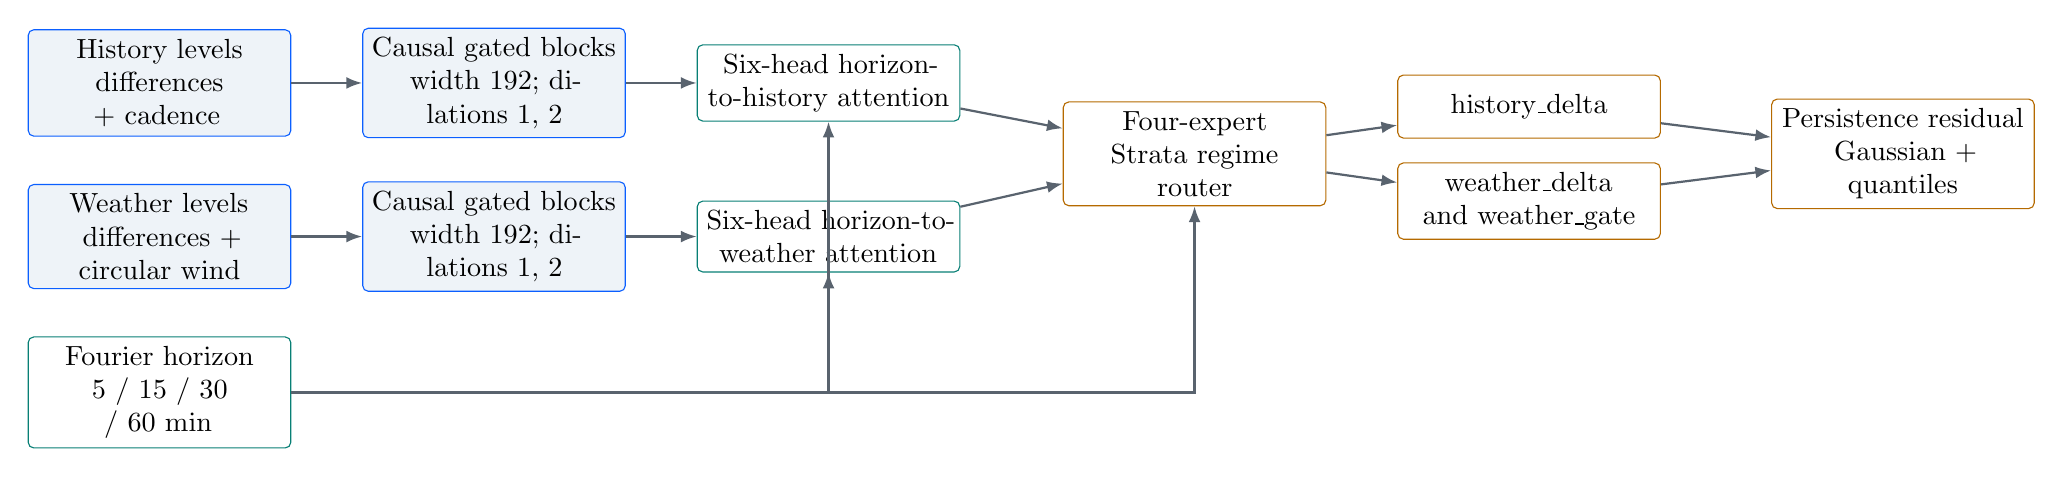
\begin{tikzpicture}[
  node distance=6mm and 9mm,
  box/.style={draw=stratagray, rounded corners=2pt, align=center,
              minimum height=8mm, text width=31mm, fill=white},
  branch/.style={box, draw=stratablue, fill=stratalight},
  query/.style={box, draw=stratateal, fill=white},
  outputbox/.style={box, draw=strataamber, fill=white},
  arrow/.style={-{Latex[length=2mm]}, thick, draw=stratagray}
]
\node[branch] (histin) {History levels\\differences + cadence};
\node[branch, below=of histin] (weatherin) {Weather levels\\differences + circular wind};
\node[query, below=of weatherin] (horizon) {Fourier horizon\\5 / 15 / 30 / 60 min};

\node[branch, right=of histin] (histenc) {Causal gated blocks\\width 192; dilations 1, 2};
\node[branch, right=of weatherin] (weatherenc) {Causal gated blocks\\width 192; dilations 1, 2};

\node[query, right=of histenc] (histattn) {Six-head horizon-to-history attention};
\node[query, right=of weatherenc] (weatherattn) {Six-head horizon-to-weather attention};

\node[outputbox, right=13mm of histattn, yshift=-9mm] (router) {Four-expert\\Strata regime router};
\node[outputbox, right=of router, yshift=6mm] (historydelta) {history\_delta};
\node[outputbox, right=of router, yshift=-6mm] (weatherdelta) {weather\_delta\\and weather\_gate};
\node[outputbox, right=14mm of weatherdelta, yshift=6mm] (head) {Persistence residual\\Gaussian + quantiles};

\draw[arrow] (histin) -- (histenc);
\draw[arrow] (weatherin) -- (weatherenc);
\draw[arrow] (histenc) -- (histattn);
\draw[arrow] (weatherenc) -- (weatherattn);
\draw[arrow] (horizon.east) -| (histattn.south);
\draw[arrow] (horizon.east) -| (weatherattn.south);
\draw[arrow] (histattn) -- (router);
\draw[arrow] (weatherattn) -- (router);
\draw[arrow] (horizon.east) -| (router.south);
\draw[arrow] (router) -- (historydelta);
\draw[arrow] (router) -- (weatherdelta);
\draw[arrow] (historydelta) -- (head);
\draw[arrow] (weatherdelta) -- (head);
\end{tikzpicture}
}
\caption{Frozen Horizon v1 information flow. The weather contribution is
hard-zeroed in the history-only arm rather than represented by a learned
missing token.}
\end{figure}

\subsection{Inputs and causal branch encoders}

The history branch tokenizes the \cn{} level, its first difference, and the
elapsed-cadence ratio. The weather branch tokenizes seven levels---wind
direction sine and cosine, speed, pressure, temperature, relative humidity,
and dew point---plus their first differences. Train-only imputation and
normalization precede both branches.

Each branch projects to width 192 and applies gated causal temporal blocks
with kernel size 3 and dilations 1 and 2. Causal padding is a correctness
constraint even though only six context rows are present: no representation
at time \(t\) may depend on a later context token.

\subsection{Horizon queries and regime fusion}

Forecast minutes are represented with fixed Fourier sine/cosine features and
a learned width-192 projection. The resulting horizon query separately
attends to history and weather with six heads. This follows the general
context-alignment motivation of MQTransformer \cite{eisenach2022mqtransformer}
while preserving the endogenous/exogenous distinction emphasized by TimeXer
\cite{wang2024timexer}.

The two attended summaries and the horizon state enter the existing
four-expert Strata regime router. The router is retained to test the
project-specific inductive bias; it is not presented as a new mixture-of-
experts concept.

\subsection{Interpretable forecast and uncertainty}

The point location is frozen as
\begin{equation}
\widehat y =
y_{\mathrm{last}} +
\Delta_{\mathrm{history}} +
\sigma(g_{\mathrm{weather}})\Delta_{\mathrm{weather}}.
\end{equation}
For the history-only arm,
\(\Delta_{\mathrm{weather}}\) and the applied weather contribution are
hard-zeroed. The design logs the last-value anchor, both deltas, the weather
gate, and regime weights for every prediction.

The existing Gaussian scale and 0.10/0.50/0.90 quantile machinery is retained.
The explicit residual supplies the location; the fused state supplies
positive scale and learned quantile offsets. A single positive scale
multiplier is fit on the pooled calibration role and then frozen before
assessment. This keeps the feature and architecture comparisons from being
confounded by a new distribution family.

\section{Alternatives considered and rejected}

\begin{description}
\item[PatchTST.] Patching is compelling for long look-back windows
\cite{nie2023patchtst}; six context rows do not provide enough temporal extent
to justify patch tokenization.
\item[TiDE replacement.] TiDE is efficient and covariate-aware
\cite{das2024tide}, which makes the compact MLP an important control. Replacing
the custom model with TiDE would not test the planned branch and weather-gate
inductive bias.
\item[Full TFT.] TFT already combines multiple input types, gating, attention,
and quantiles \cite{lim2020tft}. Its broader machinery is unnecessary for a
single site, six historical rows, no static covariates, and no known-future
weather.
\item[TimeXer reproduction.] TimeXer is the closest exogenous-variable
architecture \cite{wang2024timexer}, but its patch/global-token design targets
longer multivariate sequences. The experiment retains its conceptual
separation while using a smaller causal encoder and explicit persistence
residual.
\item[All 87 MLO fields.] This arm is rejected on evidence quality. Covariances,
QC flags, counts, and diagnostics may encode target construction or instrument
health and are not required to answer whether operational weather adds value.
\end{description}

\section{Failure modes and diagnostic obligations}

\begin{itemize}
\item \textbf{Persistence dominance.} A complex model may underperform the
latest observed value, especially at 5 minutes. This is a valid null result.
\item \textbf{Weather gate collapse.} Gates near zero across horizons support
the conclusion that these surface-weather inputs add little beyond recent
\cn{} history. Gates near one without RMSE benefit indicate uncontrolled
weather residuals rather than useful attribution.
\item \textbf{Proxy contamination.} The raw feature audit must remain
descriptive and training-only; excluded fields cannot migrate into a learned
arm.
\item \textbf{Horizon aliasing.} Timestamp checks must reject missing-row
examples whose elapsed time is inconsistent with the nominal horizon.
\item \textbf{Calibration pooling.} A pooled scalar may conceal
horizon-specific miscalibration. Coverage and CRPS must therefore be reported
at every horizon.
\item \textbf{Small assessment block.} The assessment role spans less than two
days. The preregistered circular 24-hour moving-block bootstrap respects local
dependence but cannot manufacture independent weather regimes; this limits
claim strength even if its interval is positive.
\item \textbf{Router interpretation.} Expert weights are diagnostics, not
identified physical regimes. The report must avoid causal regime labels.
\end{itemize}

\section{Claim-to-evidence map before training}

\begin{tabularx}{\linewidth}{>{\bfseries}p{0.29\linewidth}X}
\toprule
Potential claim & Required evidence\\
\midrule
Operational weather adds forecast information
& Weather Horizon v1 beats hard-zero history Horizon v1 under the frozen
point, bootstrap, seed, calibration, and regression rules.\\
Horizon v1 uses weather better than controls
& It also beats the stronger operational-weather MLP/LightGBM comparator
without material bias, tail, CRPS, or stability regression.\\
The architecture is novel
& \textbf{Not supported or claimed.} The review supports only ``custom
adaptation'' language.\\
The result generalizes
& \textbf{Not supported.} One site and a development assessment block cannot
establish cross-site, cross-instrument, or seasonal generalization.\\
The model should be promoted
& \textbf{Prohibited.} Official MLO test evidence and human approval would
still be required.\\
\bottomrule
\end{tabularx}

\section{Frozen conclusion}

The literature justifies an honest, bounded test of Horizon v1 but does not
justify an a priori performance claim. The architecture is intentionally
small, persistence-anchored, separable by information source, and instrumented
for component diagnostics. Its value will be determined solely by the frozen
MLO selection/calibration/assessment protocol. A partial or null result is
scientifically useful and must not start an assessment-driven redesign loop.

\begingroup
\small
\bibliographystyle{plain}
\bibliography{../../../research/references}
\endgroup

\end{document}
